\documentclass[a4paper,11pt]{article}
\usepackage[11pt]{extsizes}




\usepackage{cmap}					% поиск в PDF
\usepackage{mathtext} 				% русские буквы в формулах
\usepackage[T2A]{fontenc}			% кодировка
\usepackage[utf8]{inputenc}			% кодировка исходного текста
\usepackage[english,russian]{babel}	% локализация и переносы
\usepackage{ulem}                   % зачеркнутый текст
\usepackage{amssymb}			% пакет математики
\usepackage{float}
\usepackage{amsmath}
\usepackage{graphicx}
\DeclareGraphicsExtensions{.png}

%%% Страница
%\usepackage{extsizes} % Возможность сделать 14-й шрифт
\usepackage[left=1cm,right=1cm,top=1cm,bottom=1cm]{geometry} % Простой способ задавать поля
\pagestyle{empty}

\begin{document}


\begin{center}
ФЕДЕРАЛЬНОЕ ГОСУДАРСТВЕННОЕ ОБРАЗОВАТЕЛЬНОЕ БЮДЖЕТНОЕ УЧРЕЖДЕНИЕ ВЫСШЕГО ОБРАЗОВАНИЯ

    \textbf{«ФИНАНСОВЫЙ УНИВЕРСИТЕТ ПРИ ПРАВИТЕЛЬСТВЕ РОССИЙСКОЙ ФЕДЕРАЦИИ»}

Факультет информационных технологий и анализа больших данных

Департамент анализа данных и машинного обучения

\textit{
	\textbf{Дисциплина: «Теория вероятностей и математическая статистика»}}

\textit{Направление подготовки: 01.03.02 «Прикладная математика и информатика»}

\textit{Профиль: «Анализ данных и принятие решений в экономике и финансах»}

\textit{Форма обучения очная, учебный 2020/2021 год, 4 семестр}

\textbf{Билет 111}

\end{center}

\begin{enumerate}


\item

Дайте определение случайной величины, которая имеет гамма-распределение $\Gamma(\alpha,  \lambda)$, и выведите основные свойства гамма-расределения. Запишите формулы для математичсекого ожидания
$\mathbb{E}(X)$ и дисперсии $\mathbb{V}ar(X)$ гамма-распределения


\item



Случайные величины $X$ и $Y$ независимы и имеют равномерное
распределение на отрезках $[0;1]$ и $[0;10]$ соответственно. Для случайной величины $Z=\frac{Y}{X}$ найдите: 
1) функцию распределения $F_Z(x)$;
2) плотность распределения $f_Z(x)$ и постройте график плотности;
3) вероятность $\P(2,\!96\leqslant Z\leqslant 17,\!91)$.


\item


%\folder 2.pdf
(10) Известно, что доля возвратов по кредитам в банке имеет распределение $F(x) = x ^{\beta}, 0 \leqslant x \leqslant 1$.
Наблюдения показали, что в среднем она составляет $75,0\%$. Методом моментов оцените параметр $\beta$ и
вероятность того, что она опуститься ниже $20\%$


\item


(10) В группе $\Omega$ учатся студенты:$\omega _{1}...\omega _{25}$ . Пусть $X$ и $Y$ – 100-балльные экзаменационные оценки по
математическому анализу и теории вероятностей. Оценки $\omega _{i}$ студента обозначаются: $x _{i} = X(\omega _{i})$ и $y _{i} = Y(\omega _{i})$, $i = 1...25$. Все оценки известны
$x _{0} = 64, y _{0} = 84$, $x _{1} = 82, y _{1} = 42$, $x _{2} = 51, y _{2} = 99$, $x _{3} = 68, y _{3} = 57$, $x _{4} = 90, y _{4} = 71$, $x _{5} = 89, y _{5} = 55$, $x _{6} = 55, y _{6} = 55$, $x _{7} = 90, y _{7} = 58$, $x _{8} = 61, y _{8} = 78$, $x _{9} = 38, y _{9} = 84$, $x _{10} = 56, y _{10} = 95$, $x _{11} = 86, y _{11} = 69$, $x _{12} = 71, y _{12} = 72$, $x _{13} = 35, y _{13} = 99$, $x _{14} = 82, y _{14} = 67$, $x _{15} = 79, y _{15} = 59$, $x _{16} = 83, y _{16} = 88$, $x _{17} = 45, y _{17} = 75$, $x _{18} = 70, y _{18} = 79$, $x _{19} = 89, y _{19} = 80$, $x _{20} = 33, y _{20} = 30$, $x _{21} = 63, y _{21} = 73$, $x _{22} = 55, y _{22} = 53$, $x _{23} = 31, y _{23} = 78$, $x _{24} = 50, y _{24} = 90$
Требуется
найти следующие условные эмпирические характеристики: 1) ковариацию $X$ и $Y$ при условии, что одновременно $X \geqslant 50$
 и $Y \geqslant 50$; 2) коэффициент корреляции $X$ и $Y$ при том же условии.


\item

    
    	Распределение результатов экзамена в некоторой стране с $11$-балльной системой оценивания задано следующим образом:
    	$\left\{ 1 : 13, \  2 : 3, \  3 : 14, \  4 : 9, \  5 : 6, \  6 : 15, \  7 : 1, \  8 : 22, \  9 : 17, \  10 : 10, \  11 : 16\right\}$

	Работы будут перепроверять $6$ преподавателей, которые разделили все имеющиеся работы между собой случайным образом. Пусть $\overline{X}$ - средний балл (по перепроверки) работ, попавших к одному преподавателю.

	Требуется найти матожидание и стандартное отклонение среднего балла работ, попавших к одному преподавателю, до перепроверки.
    

\item


(10) Пусть $X _{1}$, $X _{2}$, $X _{3}$, $X _{4}$ выборка из $N(\theta, \sigma ^{2})$. Рассмотрим две оценки параметра $\theta$:
\[\hat \theta _{1} = \frac{3X _{1} + X _{2} + 4X _{3} + 2X _{4}}{10}, \hat \theta _{1} = \frac{X _{1} + 6X _{2} + 2X _{3} + X _{4}}{10}\]
a) Покажите, что обе оценки несмещенные.
б) Какая из оценок оптимальная?


\end{enumerate}

\begin{figure}[H]
	Подготовил
	\hfill
	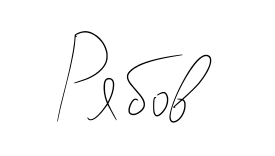
\includegraphics[width=2cm]{Prepared}
	П.Е. Рябов
\end{figure}


\begin{figure}[H]
	Утверждаю:\\
	Первый заместитель\\
	руководителя департамента\\
	Дата 01.06.2021
	\hfill
	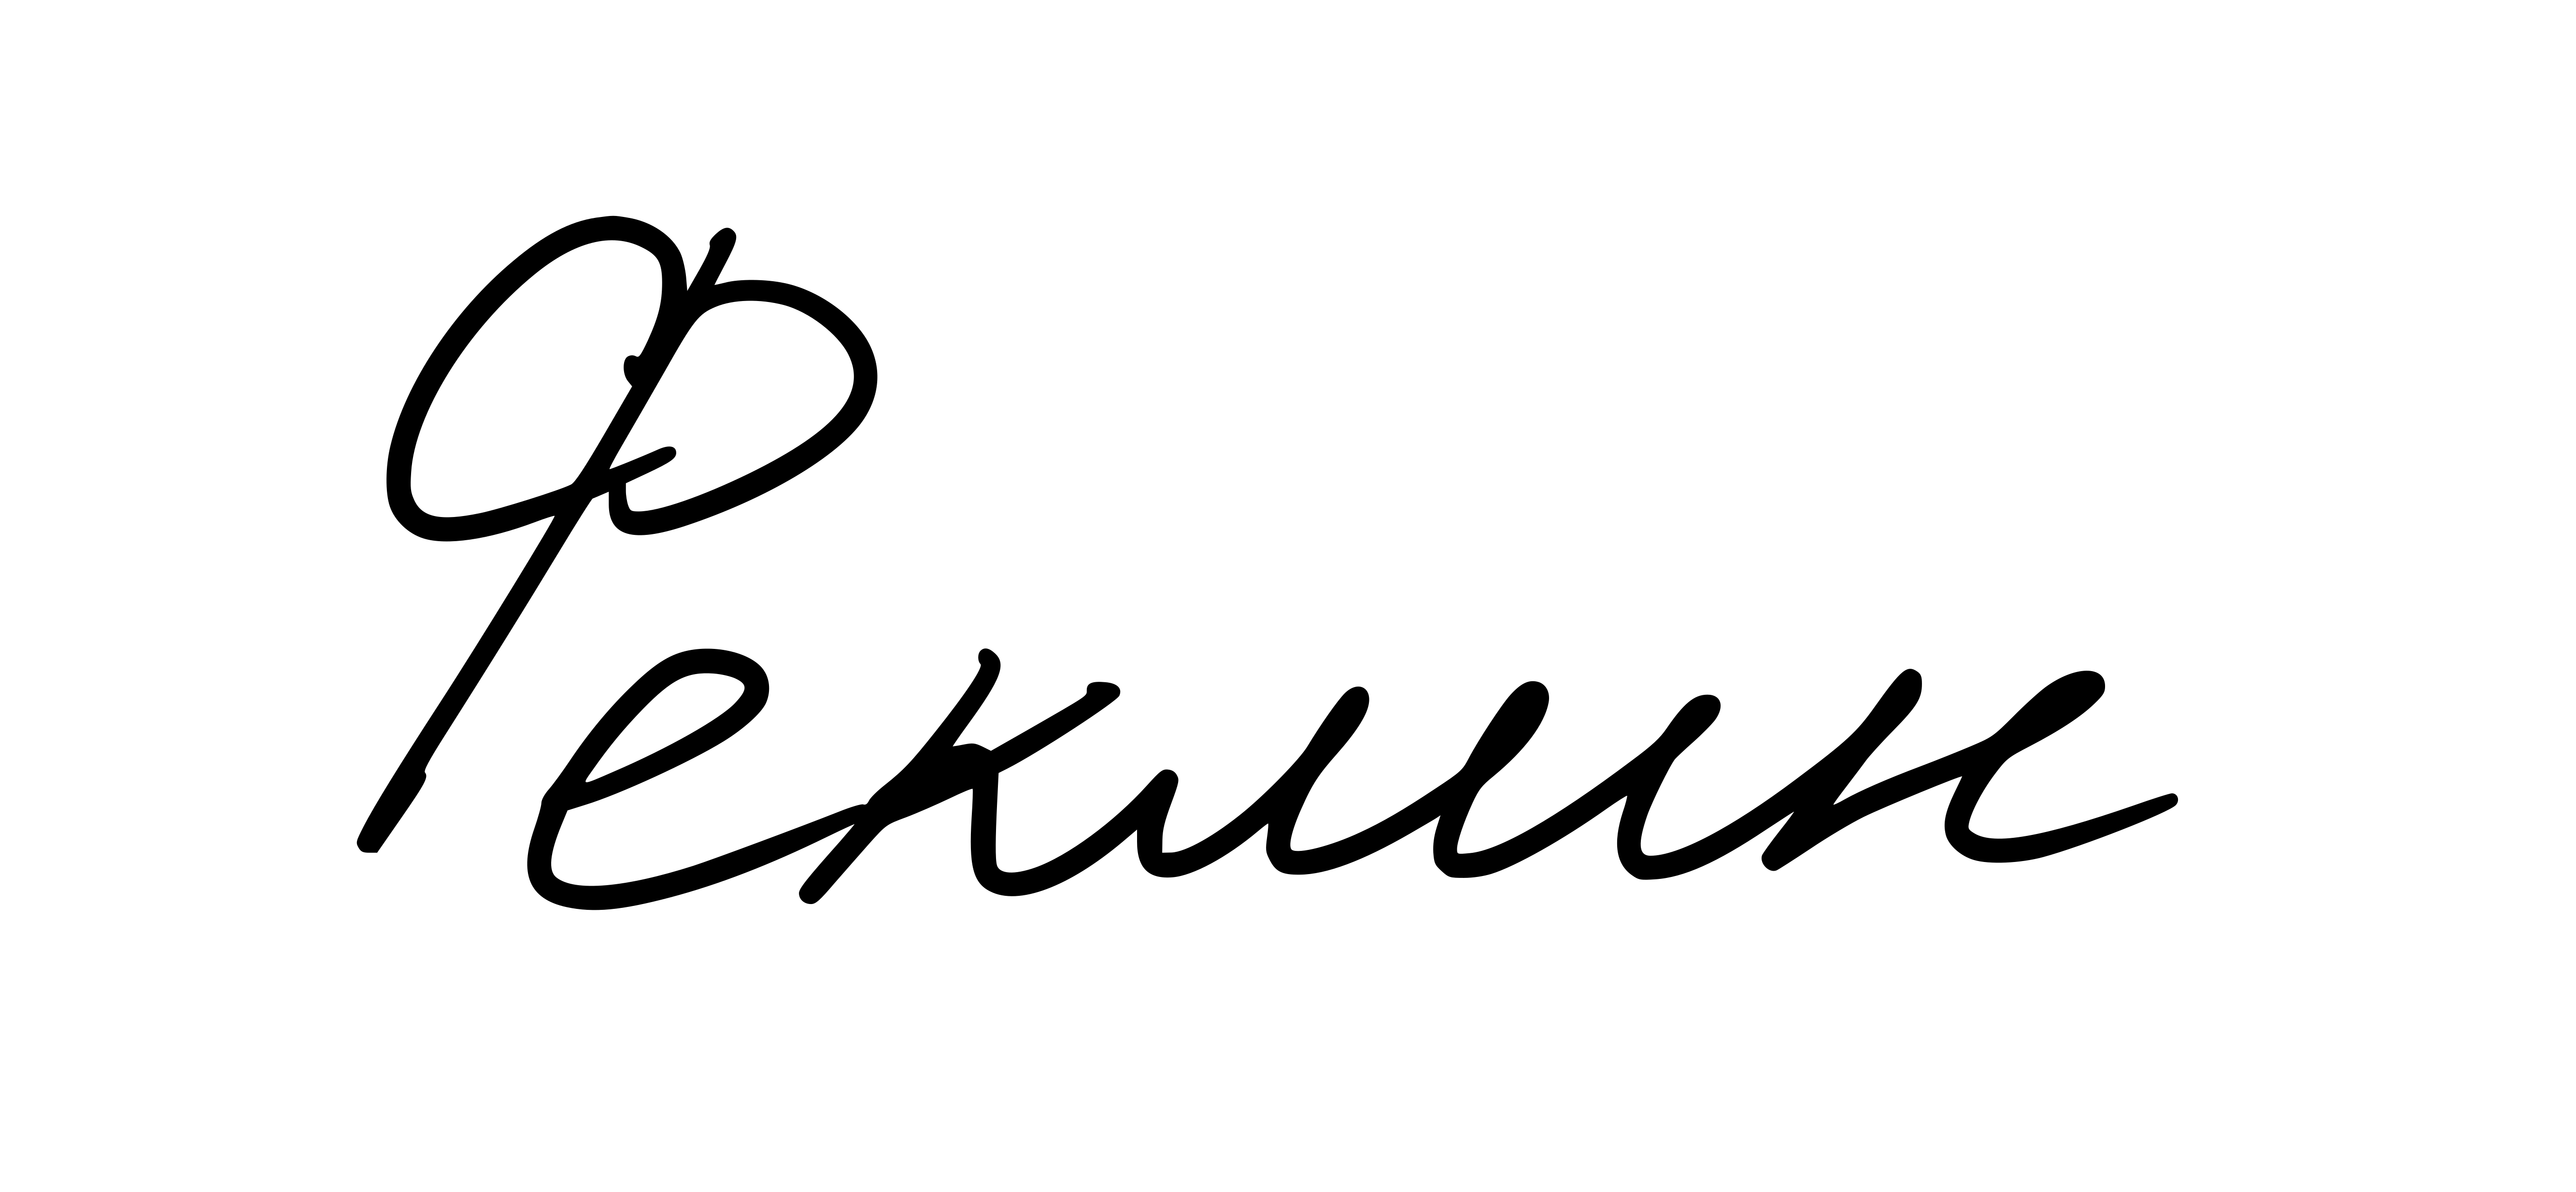
\includegraphics[width=2cm]{Approved}
	Феклин В.Г.
\end{figure}

\end{document}

